% Derived from the template file for the LaTeX package SVJour3
% for Springer journals.          Springer Heidelberg 2010/09/16
%
% This template includes a few options for different layouts and
% content for various journals. Please consult a previous issue of
% your journal as needed.
%
% First comes an example EPS file -- just ignore it and
% proceed on the \documentclass line
% your LaTeX will extract the file if required
\begin{filecontents*}{example.eps}
%!PS-Adobe-3.0 EPSF-3.0
%%BoundingBox: 19 19 221 221
%%CreationDate: Mon Sep 29 1997
%%Creator: programmed by hand (JK)
%%EndComments
gsave
newpath
  20 20 moveto
  20 220 lineto
  220 220 lineto
  220 20 lineto
closepath
2 setlinewidth
gsave
  .4 setgray fill
grestore
stroke
grestore
\end{filecontents*}
%
\RequirePackage{fix-cm}
%
%\documentclass{svjour3}                     % onecolumn (standard format)
%\documentclass[smallcondensed]{svjour3}     % onecolumn (ditto)
\documentclass[smallextended]{svjour3}       % onecolumn (second format)
%\documentclass[twocolumn]{svjour3}          % twocolumn
%
\smartqed  % flush right qed marks, e.g. at end of proof
%
\usepackage{graphicx}
%
% \usepackage{mathptmx}      % use Times fonts if available on your TeX system
%
% insert here the call for the packages your document requires
\usepackage{amsmath}
\usepackage{amssymb}
\usepackage{array}
\usepackage{hhline}
\usepackage{mathtools}
\usepackage{multirow}
\usepackage{tikz}
\usetikzlibrary{arrows, calc, decorations.pathreplacing, positioning,
  shapes.geometric}
% etc.

\usepackage{attrib}
\usepackage{csquotes}

\usepackage{graphicx}
\graphicspath{ {support/} }

% please place your own definitions here and don't use \def but
% \newcommand{}{}

\newcommand{\etal}{{\em et al.}}
\newcommand{\Bagai}{Bagai \etal{}}

% For example theory of lists
\newcommand{\function}{\rightarrow}
\newcommand{\Zero}{\text{Z}}
\newcommand{\Succ}{\text{S}}
\newcommand{\List}{\text{List}}
\newcommand{\ListA}{\text{List} \  a}
\newcommand{\Nil}{\text{Nil}}
\newcommand{\Cons}{\text{Cons}}
\newcommand{\Head}{\text{head}}
\newcommand{\Tail}{\text{tail}}
\newcommand{\Append}{\text{append}}
\newcommand{\Reverse}{\text{reverse}}
\newcommand{\Length}{\text{length}}
\newcommand{\Map}{\text{map}}
\newcommand{\Foldl}{\text{foldl}}
\newcommand{\Foldr}{\text{foldr}}

% For interestingness table
\newcommand{\iE}{\textbf{E}}
\newcommand{\iN}{\textbf{N}}
\newcommand{\iS}{\textbf{S}}
\newcommand{\iA}{\textbf{A}}
\newcommand{\iC}{\textbf{C}}
\newcommand{\iU}{\textbf{U}}
\newcommand{\tIFF}{if-and-only-if}
\newcommand{\tNE}{non-exists}
\newcommand{\tIMP}{implies}
\newcommand{\tEQ}{equations}
\newcommand{\tINE}{inequalities}
\newcommand{\tCON}{conditional}
\newcommand{\tRow}[1]{#1 \\ \hline}

% Insert the name of "your journal" with
\journalname{Journal of Automated Reasoning}

\begin{document}

\title{Quantitative Benchmarking for Automatically Generated Conjectures%\thanks
% {Grants or other notes about the article that should go on the front page
% should be placed here. General acknowledgments should be placed at the end of
% the article.}
}
% \subtitle{Do you have a subtitle?\\ If so, write it here}

% \titlerunning{Short form of title}        % if too long for running head

\author{Chris Warburton \and
        Alison Pease    \and
        Jianguo Zhang
        % TODO: Invite Katya? Even if she only offers some help, can acknowledge
}

% \authorrunning{Short form of author list} % if too long for running head

\institute{C. Warburton \at
           University of Dundee \\
           \email{c.m.warburton@dundee.ac.uk}           %  \\
%             \emph{Present address:} of F. Author  %  if needed
           \and
           A. Pease \at
           University of Dundee \\
           \email{a.pease@dundee.ac.uk}
           \and
           J. Zhang \at
           University of Dundee \\
           \email{j.n.zhang@dundee.ac.uk}
}

\date{Received: date / Accepted: date}
% The correct dates will be entered by the editor

\maketitle

% Look carefully at each system's (paper's) eval section

% Make it clear that methodology is the point (it's not just a detail, like in a
% chemistry paper for example)

\begin{abstract}
  We propose a benchmark suite for evaluating the efficiency and effectiveness
  of \emph{conjecture formation} by automated tools for \emph{mathematical
    theory exploration} in higher-order, inductive theories; a domain especially
  suited for analysing software. By providing standard tools and metrics, we
  hope to encourage innovation and comparison between the disparate approaches
  currently being pursued, and spur improvements similar to those seen in the
  competitive field of automated theorem proving.
%\keywords{First keyword \and Second keyword \and More}
% \PACS{PACS code1 \and PACS code2 \and more}
% \subclass{MSC code1 \and MSC code2 \and more}
\end{abstract}

\section{Introduction}
\label{intro}

% Lay out the field of TE: motivation, systems, evaluation, problems...

\emph{Conjecture generation/formation}, a sub-field of \emph{mathematical theory
  exploration} (MTE), is the open-ended problem of producing conjectures about a
given logical theory which are somehow ``interesting''.

This has applications wherever we find use for formal statements: in proof
assistants and their libraries, in mathematics education and research, and in
the specification, verification, optimisation and testing of software.

Existing attempts at tackling this problem are difficult to compare, due
partially to the variety of approaches taken, but also because of the inherent
ambiguity of the task and the different goals emphasised by their designers and
their choice of evaluation method.

We attempt to solve this discrepancy, at least for the foreseeable future, by
defining a standard, unambiguous benchmarking approach with which to compare
the conjecture generation of MTE systems. Our contributions include:

\begin{itemize}
\item A general methodology for benchmarking conjecture generation.
\item Resolving the issue of ``interestingness'' through the use of
  theorem-proving benchmarks as a ground-truth.
\item A specific instantiation of this methodology, using the Tons of Inductive
  Problems benchmark as a corpus.
\item Automated tooling to perform this benchmarking.
\item Application of our methodology to the QuickSpec MTE system, and a
  discussion of the results.
\end{itemize}

Section \ref{sec:background} describes MTE and the conjecture generation problem
in more detail, along with existing approaches and their evaluation
methodologies. We explain our proposal for a more general benchmark in section
\ref{sec:proposal} and section \ref{sec:application} shows the results when
applied to existing MTE tools. Analysis of these results is given in section
\ref{sec:discussion} and concluding remarks in \ref{sec:conclusion}.

%- Existing approaches are difficult to compare
% - They want different things
% - They're evaluated differently
% - They're evaluated ``locally'' (as white boxen)

% Look at phd symposium 2017, moa's conjecture synthesis paper, etc.
% We can just jump straight in to automated conjecture generation

\section{Background}
\label{sec:background}

\subsection{Motivation}
\label{sec:motivation}

% more detail about evaluation, interestingness, etc. Reference Simon/Alan
% interestingness, e.g. examples from textbooks, etc.

\begin{figure}
  \begin{equation*}
    \begin{split}
      \forall a. \Nil            &: \ListA                                  \\
      \forall a. \Cons           &: a \rightarrow \ListA \rightarrow \ListA \\
      \Head(\Cons(x, xs))        &= x                                       \\
      \Tail(\Cons(x, xs))        &= xs                                      \\
      \Append(\Nil,         ys)  &= ys                                      \\
      \Append(\Cons(x, xs), ys)  &= \Cons(x, \Append(xs, ys))               \\
      \Reverse(\Nil)             &= \Nil                                    \\
      \Reverse(\Cons(x, xs))     &= \Append(\Reverse(xs), \Cons(x, \Nil))   \\
      \Length(\Nil)              &= \Zero                                   \\
      \Length(\Cons(x, xs))      &= \Succ (\Length(xs))                     \\
      \Map(f, \Nil)              &= \Nil                                    \\
      \Map(f, \Cons(x, xs))      &= \Cons(f(x), \Map(f, xs))                \\
      \Foldl(f, x, \Nil)         &= x                                       \\
      \Foldl(f, x, \Cons(y, ys)) &= \Foldl(f, f(x, y), ys)                  \\
      \Foldr(f, \Nil,         y) &= y                                       \\
      \Foldr(f, \Cons(x, xs), y) &= f(x, \Foldr(f, xs, y))
    \end{split}
  \end{equation*}
  \caption{A simple theory defining a $\List$ type and some associated
    operations, taken from~\cite{Johansson.Dixon.Bundy:conjecture-generation}.
    $\Zero$ and $\Succ$ are from a Peano encoding of the natural numbers.}
  \label{figure:list_theory}
\end{figure}

Given a logical theory, such as the theory of lists shown in
Figure~\ref{figure:list_theory}, we may want to find theorems which describe its
behaviour. This could be for mathematical curiosity, or due to the theory's
importance in some domain. In particular, for theories which capture the
semantics of some software library, we may want to verify that certain
(un)desirable properties do (not) hold. We might also want to \emph{optimise}
programs using this library, rewriting expressions into a form which requires
less time, memory, network usage, etc. To avoid altering a program's result,
such rewrites should come with theorems proving their correctness, such as the
following theorem for our theory of lists:

\begin{equation} \label{eq:mapreduce}
  \forall f. \forall xs. \forall ys.
    \Map(f, \Append(xs, ys)) = \Append(\Map(f, xs), \Map(f, ys))
\end{equation}

Equation \ref{eq:mapreduce} justifies a rewrite rule for splitting a single
$\Map$ call into multiple independent calls dealing with different sections of a
list. Such rules are useful optimisations since each call can be evaluated in
parallel, leading to the ``map/reduce'' programming paradigm.

All of these example use cases require the ability to discover theorems about
some particular theory. This is a hard problem in general, but presents
opportunities for automation due to the precise, symbolic nature of the domain.

\subsection{Automating Construction and Exploration of Theories}
\label{sec:te}

The task of discovering theorems in an arbitrary theory can be
described as the interplay of several processes: (i) formulating new
definitions and concepts; (ii) finding patterns suitable for posing as
conjectures; and (iii) proving that those conjectures are theorems.
The latter is studied extensively in the field of Automated Theorem
Proving (ATP). Far less attention has been paid to automating the
first two tasks, which both Automated Theory Formation (ATF) and
Mathematical Theory Exploration (MTE) address.  We discuss the relationship
between ATF and ATE in historical context in
$\S$\ref{exploration-versus-formation}.

A major challenge for both ATF and MTE is choosing how to narrow down
the set of generated conjectures to those deemed ``interesting'', since this is
an imprecise term with many different interpretations. For example, all existing
approaches agree that simple tautologies are ``uninteresting'', but differ when
it comes to more complex statements.  Colton \etal{} give a survey of systems for
theory formation and exploration, and their notions of ``interestingness'' for
concepts and conjectures, identifying six notions in
total~\cite{colton2000notion}. These notions, as applied to conjectures, are:

{\bf Empirical plausibility}, which checks whether a property holds
across some specific examples. This is especially useful for avoiding
false conjectures, without resorting to a full proof search.

{\bf Novelty} is whether a conjecture, or one isomorphic or more
general, has already been seen.

{\bf Surprisingness} of a conjecture is whether or not it is
``obvious'', for example if it is an instance of a tautology.

{\bf Applicability} depends on the number of models in which a
conjecture holds. The system of \Bagai{} conjectures the non-existence of
objects, and hence favours statements with zero applicability. Other systems
treat applicability as a positive aspect: the more applicable the statement, the
more interesting it is.

{\bf Comprehensibility} depends on the complexity of a statement. Simpler
statements are considered more interesting, hence many of the systems explore
simpler/smaller statements before complex/larger ones, to more efficiently find
those which are interesting.

{\bf Utility} is the relevance or usefulness of a conjecture to the
user's particular task. For example, if we want to find optimising
rewrite rules such as equation 1, then utility would include whether
or not a conjecture justifies a rewrite rule, the difference in
resource usage of the expressions involved, and how common those
expressions are in real usage.


\begin{table}
  \centering
  \begin{tabular}{ |l|l|c|c|c|c|c|c| }
    \hline
    \multirow{2}{*}{\textbf{Program}}                     &
    \multirow{2}{*}{\textbf{Conjecture Types}}            &
    \multicolumn{6}{c}{\textbf{Interestingness Measures}} \\ \hhline{~~------}
    \tRow{          &                    & \iE & \iN & \iS & \iA & \iC & \iU}
    \tRow{AM        & \tIFF, \tIMP, \tNE &   X &   X &   X &   X &   X &   X}
    \tRow{GT        & \tIFF, \tIMP, \tNE &   X &   X &   X &   X &   X &   X}
    \tRow{Graffiti  & \tINE              &   X &   X &   X &     &   X &   X}
    \tRow{\Bagai{}  & \tNE               &     &   X &     &   X &   X &    }
    \tRow{HR        & \tIFF, \tIMP, \tNE &   X &   X &   X &   X &   X &   X}
    \tRow{QuickSpec & \tEQ               &   X &   X &     &   X &   X &    }
    \tRow{Speculate & \tCON \tEQ / \tINE &   X &   X &     &   X &   X &    }
    \tRow{IsaCoSy   & \tEQ               &   X &   X &     &   X &   X &   X}
    \tRow{IsaScheme & \tEQ               &   X &   X &     &   X &   X &   X}
  \end{tabular}
  \caption{Classification of MTE systems from \cite{colton2000notion}, extended
    to those compared in \cite{claessen2013automating} (QuickSpec is the
    conjecture generation component of HipSpec). The interestingness measures
    are \iE{}mpirical plausibility, \iN{}ovelty, \iS{}urprisingness,
    \iA{}pplicability, \iC{}omprehensibility (low complexity) and \iU{}tility.}
  \label{table:colton}
\end{table}

% JUSTIFICATIONS
%
% IsaCoSy uses counter-example checking; this ensures empirical plausibility
% IsaCoSy uses constraints to avoid special-cases; this ensures novelty
% IsaCoSy uses utility, since there are some hard-coded patterns which are
% looked for
%
% Speculate uses a form of unification to ensure novelty, making sure one
% equation is not a special-case of another
% Speculate uses LeanCheck to enumerate values, looking for counterexamples
% Speculate uses testing, to ensure Empirical Plausibility
%
% QuickSpec uses QuickCheck to ensure empirical plausibility
% QuickSpec uses a congruence closure algorithm to ensure novelty
%
% IsaScheme uses utility, since it determines the "quality" of a definition
% based on how many theorems it appears in?
% IsaScheme uses novelty, using an equational rewrite system (Knuth-Bendix
% completion) to remove redundancies
% IsaScheme uses utility, since it focuses on the terms and definitions of a
% user's theory. However, don't all of them?
% IsaScheme uses counterexample checking for empirical plausibility.

% ONLY APPLIES TO PRECONDITIONS
% APPLICABILITY: ensure a conjecture holds in many models (or exactly zero, in
% the case of Bagai et al). Does the testing-based approach of QuickSpec and
% Speculate ensure that there's a model? After all, these are concrete values
% rather than e.g. implications of some abstract specification.

We summarise the criteria in Table 1 and state which were used in key
ATF/MTE systems. The entries for AM, GT, Graffiti, \Bagai{} and HR are based
on this survey (the latter is Colton's own system). We extend this analysis to
some more recent systems in the remaining rows (based on our understanding of
their function): QuickSpec, Speculate~\cite{braquehais2017speculate}, IsaCoSy
and IsaScheme.

The latter systems all use testing to check for counterexamples, which ensures
results are empirically plausible and applicable (conditions are satisfiable,
types are inhabited, etc.). They also use a small-to-large search order,
ensuring more easily-comprehensibile conjectures are explored first.

IsaCoSy ensures novelty using a constraint system, such that no generated
expression can be simplified using a previously-found equation. The other
systems use post-hoc filters based on unification and term rewriting to discard
expressions or equations which are special-cases of some other, more general
result.

IsaCoSy is able to look for commonly desirable patterns, such as commutativity
and associativity, which increases the utility of its output, whilst IsaScheme
is completely based around such pattern-instantiation.

This diversity of approaches makes it difficult to compare the existing
evaluations of these systems directly. In particular, evaluation methods created
for one system might not make sense for another, due to assumptions made about
the algorithms' operation. For example, the novelty filters used by QuickSpec
and Speculate are applied to the whole output set, guaranteeing that no
special-cases will appear; yet we cannot assume this in the case of IsaCoSy,
since its constraint solver allows special cases if they're found \emph{before}
the general case (it does not go back and discard previous results).

With such ambiguous and varied goals, approaches and assessment criteria it is
difficult to compare MTE systems in a quantitative way, and hence to form some
measure of ``progress'' for the field. Our proposed benchmarking methodology
attempts to remedy this by setting a clear target, hopefully in line with the
myriad goals of existing researchers, whilst being generally applicable to
systems of this type.

\section{Theory Exploration versus Theory
  Formation}\label{exploration-versus-formation}

In this section we put the Mathematical Theory Exploration approach
into context both historically, and with respect to related approaches
such as in Automated Theory Formation systems.

\subsection{A Short History of Automated Mathematics}

\begin{quote}
...``in his subsequent design for an Analytical Engine Mr. Babbage has
shown that material machinery is capable, in theory at least, of
rivalling the labours of the most practised mathematicians in all
branches of their science.'' \cite[p. 498]{jevons}
\end{quote}

The first automated mathematical system, the mechanical calculator
(known as the Pascaline), was an adding machine that could perform
additions and subtractions directly and multiplication and divisions
by repetitions, and was conceived by Pascal in 1642 while reorganising
tax revenues \cite{d'ocagne}. Subsequent early systems include
M\"uller's universal calculating machine in 1784, which he built for
the purpose of calculating and printing numerical tables: he invented
this when he had to check and recalculate some tables relating to the
volumes of trees \cite[p. 65]{lindgren}. Thirty seven years later,
Babbage invented his famous difference engine: an automatic,
mechanical calculator designed to tabulate polynomial functions. This
was inspired by a flawed table of logarithms and the idea that
machines would be quicker and more reliable \cite{bowden}. It is
interesting to note background and motivation: while Pascal and
Babbage were mathematicians, with an interest in engineering, M\"uller
was an engineer with an interest in mathematical knowledge. All three
systems were conceived as an aid to mathematicians, as well as
scientists, accountants and surveyors.

Differences in background and motivation continue to be relevant
today. While the majority of work in automating mathematics has been
in symbolic manipulation and theorem proving, we are concerned here
with other aspects of mathematics, including the construction of conjectures,
(counter\nobreakdash-)examples and theorems. These tasks, along with the
formation of new definitions and concepts, are varyingly known as
``Automated Theory Formation''~\cite{lenat:77,colton:book},
``Mathematical Theory Exploration''~\cite{buchberger:06} (also sometimes
prefaced with ``Computer-Aided'', ``Automated'' or ``Algorithm-Supported''),
``Automated Mathematical Discovery''~\cite{epstein:91,colton:interestingness,esarm2008},
``Concept Formation in Discovery Systems''~\cite{haase}, and
``Automated Theorem Discovery''~\cite{roy}. Such a plethora of terminology can
be unhelpful and can mask similarities between the different fields. In
particular, the twin strands of Automated Theory Formation and
Automated Mathematical Theory Exploration seem to be developing
somewhat independently without a clear differentiating
methodology. Below we discuss commonalities and differences between
the two schools of thought.

We limit our discussion to applications in mathematics, although there are
similar approaches being applied to the task of \emph{scientific} discovery.
Scientific knowledge relies on inductive reasoning and experimental testing,
which are not so important to a mathematical theory. However, these techniques
do play an important role in many of the tools we investigate: in particular,
inductive reasoning allows a system to conjecture statements which may be too
difficult for it to deductively prove; whilst experimental testing, e.g. by
checking universally-quantified statements against some specific values, allows
many falsehoods to be quickly discarded without requiring more elaborate
symbolic reasoning.

\subsection{Automated Theory Formation}

% 1. history of terminology
Automated theory formation derives its terminology from psychology in which the
term ``concept formation'' is used (see, for example, \cite{bruner:67}) to
describe the search for features which differentiate exemplars from
non-exemplars of various categories. Lenat used this term in his 1977 paper:
{\em Automated Theory Formation in Mathematics} \cite{lenat:77}.

% 4. example systems - AM, HR, ...
When Lenat built the AM system \cite{lenat:77}, there were systems
which could define new concepts for investigation, such as those
described in \cite{winston}, and systems which could discover
relationships among known concepts, such as Meta-Dendral
\cite{buchanan:75}. No system could perform both of these tasks: Lenat
saw this as the next step. AM was designed to both construct new
concepts and conjecture relationships between them; fully automating
the cycle of discovery in mathematics. Lenat describes this as
follows:

\begin{quote}
``What we are describing is a computer program which
defines new concepts, investigates them, notices
regularities in the data about them, and conjectures
relationships between them. This new information is used
by the program to evaluate the newly-defined concepts,
concentrate upon the most interesting ones, and iterate the
entire process.'' \cite[p. 834]{lenat:77}
\end{quote}

AM was a rule-based system which used a frame-like scheme to represent
its knowledge, enlarged its knowledge base via a collection of
heuristic rules, and controlled the firing of these rules via an
agenda mechanism. Lenat chose elementary arithmetic as the development
domain because he could use personal introspection for the heuristics
for constructing and evaluating concepts. Given the age of this
discipline, Lenat thought it unlikely that AM would make significant
discoveries, although he did cite its ``ultimate achievements'' as the
concepts and conjectures it discovered (or could have discovered). He
suggested various criteria by which his system could be evaluated,
many of which focused on an exploration of the techniques. For
instance, he considered generality (running AM in new domains) and how
finely-tuned various aspects of the program are (the agenda, the
interaction of the heuristics, etc). %most of which were qualitative.
Lenat saw his system and future developments in this field as having
implications for mathematics itself (finding results of significance),
for automating mathematics research (developing AI techniques), and
for designing ``scientist assistant'' programs (aids for
mathematicians). This shows a broad spread of motivation. Despite the
seeming success of the AM system, it is one of the most criticised
pieces of AI research. In their case study in methodology, Ritchie and
Hanna analysed Lenat's written work on AM and found that there was a
large discrepancy between his theoretical claims and the implemented
program \cite{partridge}. For instance, Lenat made claims about how AM
invented natural numbers from sets, whereas it used one heuristic
which was specifically written in order to make this connection (and
not used in any other context). Another problem was that the processes
were sometimes under-explained. For an argument of why many of the
claims made by Lenat about AM were false, see chapter 13 of
\cite{colton:book}.

\subsection{Mathematical Theory Exploration}

The phrase Mathematical Theory Exploration (MTE) is a recent term
which seems to have originated with Buchberger and colleagues (see,
for example, \cite{buchberger}). His motivation is to support
mathematicians during their exploration of mathematical theories. This
support is intended to be for the straightforward reasoning, which he
argues, covers most mathematical thought, rather than the ingenious
points, which he leaves for human mathematicians. Buchberger's long
term goal is to provide routine tools for the exploration activity of
working mathematicians, to support the invention and structured
build-up of mathematical knowledge. The Theorema project aims at
prototyping features of a system for such a purpose. These features
include Integration of the Functionality of Current Mathematical
Systems (retention of the full power of current numerics and computer
algebra systems, as well as enabling the user to add their own
algorithms to the system); Attractive Syntax (input and output is
readable and presented attractively, and can be personalised by the
user); and Structured Mathematical Knowledge Bases (tools are provided
for building and using large mathematical knowledge
libraries). Buchberger has evaluated the potential of this strategy by
illustrating the automated synthesis of his own Gr\"obner bases
algorithm \cite{buchberger:04}.

Recent systems developed in this area include MATHsAiD \cite{roy},
IsaScheme \cite{MontanoRivas2011} and IsaCosy \cite{johansson}. The
goal of the MATHsAiD (Mechanically Ascertaining Theorems from
Hypotheses, Axioms and Definitions) project is to build a tool which
takes in a set of axioms, concept definitions and a logic and applies
its inference rules to reason from the axioms to theorems. The
motivation is to produce a tool which will help mathematicians to
explore the consequences of a set of axioms or a particular concept
definition. One of the main challenges of the project has been to
automatically evaluate interestingness: to distinguish important
theorems from results which, although they follow from a set of
axioms, are of little mathematical interest.

%IsaScheme
Monta{\~n}o-Rivas \etal{} have implemented a scheme-based approach to MTE in their
IsaScheme system~\cite{MontanoRivas2011}. Schemes are higher-order formulae
which can be used to generate new concepts and conjectures; variables within the
scheme are instantiated automatically and this drives the invention process.
For instance, in the theory of natural numbers, given the concepts of successor
($suc$), addition ($+$) and zero ($0$), IsaScheme can use the following scheme
to invent the concept of multiplication:

\[
\text{def-scheme}(g,h,i,j) \equiv\\
  \exists f. \forall x y. \left\{
  \begin{array}{l l}
    f(g,y) = h (y)  \: \text{and}  & \\
    f(i(x),y) = j(y,f(x,y)) & \\
  \end{array} \right.
\]
where the existentially quantified variable $f$ stands for the new
function to be defined in terms of the variables g, h, i and j. Within
the theory of natural numbers, IsaScheme instantiates this scheme with
$\sigma_1 = \{g \mapsto 0, h \mapsto (\lambda x.0), i \mapsto suc, j
\mapsto +\}$. In this example, $f \mapsto *$ (multiplication), since:

\begin{align*}
0*y  &= 0 \\
suc(x) * y &=y + (x*y).
\end{align*}
The new multiplication function $f$ can itself be used to instantiate
variables in the same scheme, resulting in the invention of the
exponentiation concept (these examples are taken from
\cite{MontanoRivas2011}).

%IsaCosy
The IsaCosy system (Isabelle Conjecture Synthesis) is a program for
inductive theory formation, which synthesises conjectures from the
available constants and free variables. Only terms which do not
contain subterms that can be rewritten by a set of rewrite rules can
be synthesised.  Conjectures are tested by sending them to a
counterexample checker and, if no counterexamples are found, then sent
to IsaPlanner which attempts to prove them.

% Discussion.

\subsection{Commonalities and Differences between MTE and ATF}

We believe that ATF and MTE share many goals and would benefit from a
closer alignment: both fields are highly specialised and by joining
forces (while being explicit about differences) the techniques being
developed would have greater impact. This closer alignment is already
beginning to take place. The main commonalities between MTE and ATF
are that both are interested in the same aspects of mathematical
thinking, aiming to automatically construct and evaluate elements of a
mathematical theory, including concepts, conjectures, theorems, axioms
and examples. Both strands contrast themselves with Automated Theorem
Proving. The main historical differences between these two approaches
seem to be that in MTE:
\begin{itemize}
\item the main proponents define themselves as mathematicians (they
  hold a PhD and have experience in research mathematics);
\item the primary motivation is to support mathematicians;
\item systems tend to be user-interactive;
\item systems tend to be specific to mathematics,
\end{itemize}

while in ATF:

\begin{itemize}
\item the main proponents define themselves as AI researchers (they
  often have a mathematics background up to Masters level, but their
  PhD and research experience is in AI);
\item the primary motivation is to extend AI techniques; a secondary
  motivation is to produce interesting new mathematics;
\item systems tend to be fully automated;
\item systems can often be applied to non-mathematical domains.
\end{itemize}

The different backgrounds of the people who named the fields
``automated theory formation'' (Lenat) and ``mathematical theory
exploration'' (Buchberger) perhaps reflects different metaphysical
perspectives on invention (in which case new mathematical ideas are
being {\em formed}, created or produced) and discovery (in which case
abstract mathematical objects exist independently of us and are {\em
  explored} or investigated) in mathematics.\footnote{There is a vast
  literature on the Platonic and the constructivist view of
  mathematics: we shall not venture down this path here (interested
  readers are referred to \cite{hersh:97,shapiro}). Instead, for now,
  we make the pragmatic assumption that while there may well be
  different cognitive processes involved in invention than those
  involved in discovery, the fields of ATF and MTE are not currently
  concerned with this level of detail and so the philosophical
  distinction is not relevant for our purposes.} As can be seen above,
some of these historical differences are disappearing, and current
systems such as MATHsAiD \cite{roy}, IsaScheme \cite{MontanoRivas2011}
and IsaCosy \cite{johansson} are bridging the methodological gap
between ATF and MTE. This is particularly true in terms of
fully-automatic/user-interactive and the domain-specific/general
aspects.

\subsection{Existing Evaluations}
\label{sec:existing}

There are three aspects to consider when we evaluate an MTE system:

\begin{enumerate}
\item The quality of each conjecture, which is the ``interestingness'' discussed
  above.
\item The quality of the \emph{set} of conjectures produced, used for relative
  interestingness criteria like novelty, as well as to assess consistency.
\item Performance of the system, to find the balance struck between output
  quality and time taken.
\end{enumerate}

% TODO: Should "generality" be one? Or is that just an implicit "don't cheat"
% assumption?

If we limit ourselves to exploring higher-order theories with inductive types
(a domain closely matching our interest in analysing software), we do find a
direct comparison of three systems~\cite{claessen2013automating}: HipSpec,
IsaCoSy and IsaScheme. QuickSpec, shown in table \ref{table:colton}, is the
conjecture-generating component of HipSpec (which sends those conjectures into
automated theorem provers).

This comparison uses \emph{precision/recall analysis}: a particular set of
definitions is chosen, such as those in figure \ref{figure:list_theory}, and a
\emph{ground truth} is chosen as the 'ideal' set of conjectures which we would
like an MTE system to produce from these definitions.

Each system is run, and their output compared to the ground truth. To score
100\% on precision and recall, an MTE system must output all of the conjectures
which appear in the ground truth, and nothing else:

\begin{itemize}
\item \emph{Precision} is the proportion of a system's output which appears in
  the ground truth. This penalises systems which output large numbers of
  conjectures in the hope that some turn out to be ``good''.
\item \emph{Recall} is the proportion of the ground truth which appears in the
  system's output. This penalises systems which overly restrict their output to
  avoid generating ``bad'' conjectures.
\end{itemize}

Precision and recall fulfil our second requirement, by directly measuring the
quality of the \emph{set} of conjectures. Their ``interestingness'' criterion is
indirect: asking only whether or not a conjecture appears in the ground truth.
A satisfactory solution to our first requirement hence requires careful choice
of the ground truth set.

This particular analysis takes its ground truths from the standard library of
the Isabelle theorem prover, with one involving the natural numbers, and the
other involving the list functions from figure \ref{figure:list_theory}. The
library authors have gone to the effort of stating, proving and including these
theorems in every copy of their software, which is a good indication that they
are useful or important.

One problem with this choice is the small size of these libraries. For example,
the benchmark based on Isabelle/HOL's theory of natural numbers given
in~\cite{Johansson.Dixon.Bundy:conjecture-generation} contains only 4
definitions and a ground truth of 12 theorems. Whilst such benchmarks allow
objective comparisons between different approaches, their narrow scope doesn't
provide much indication of performance in different, especially \emph{novel},
domains.

\section{Theory Exploration Benchmark}
\label{sec:proposal}

Our main contribution is a benchmarking methodology, shown in figure
\ref{figure:flow_chart}, which generates both a large definition/ground-truth
corpus (an order of magnitude larger than previous work) and a scalable,
statistical approach to evaluating MTE systems using this corpus. We follow a
precision/recall approach similar to the work described above, with the main
difference being the source of definitions and ground truths: we take existing
problem sets designed for automated \emph{theorem proving}, and adapt their
content for use in the \emph{theory exploration} setting.

\subsection{Preparation}
\label{section:prep}

Automated theorem proving is an active area of research, with large problem sets
and regular competitions to prove as much as possible, as fast as
possible\cite{pelletier2002development}. These problem sets are an opportunity
for theory exploration, as their definitions and theorems can be used as a
corpus, in the same way that Isabelle libraries have been used in the past.

Some problem sets are more amenable for this purpose than others. The most
suitable are those which have the following properties:

\begin{itemize}
\item For each problem, there should be a clear distinction between the theorem
  to be proved and the definitions involved, such that the two can be easily and
  meaningfully separated. This rules out problem sets like those of
  SMT-COMP~\cite{barrett2005smt}, where many problems involve uninterpreted
  functions, whose behaviour is \emph{implicit} in the logical structure of the
  theorem statement but not separately \emph{defined}.
\item Definitions should be \emph{strongly typed}, such that they can be
  translated into the native language of each MTE system (in this work, that
  includes Haskell\iffalse FIXME and Isabelle\fi).
\item The problem set should be relevant to the desired domain. In our case, we
  desire higher-order functions and inductively defined types, which rules out
  first-order languages/logics (such as TPTP~\cite{sutcliffe2009tptp}).
\item Since it will act as our ground truth, the problem set should ideally
  contain every ``interesting'' conjecture involving its included
  definitions. Realistically, we should aim for each definition to appear in
  \emph{many} theorem statements; rather than each problem having unique
  definitions.
\item The problem set should be as large as possible, for robustness of the
  resulting statistics.
\end{itemize}

Once such a problem set has been chosen, we must separate the definitions
referenced by the theorems from the theorem statements themselves. The former
will be used as input to the MTE systems under evaluation, whilst the latter
form a ground truth corpus against which to compare the MTE output.

It is important to ensure that there are no duplicate definitions: theory
exploration does not depend on the names of functions, so neither should our
analysis. For example, consider a problem set which includes a commutativity
theorem for a \texttt{plus} function, and an associativity theorem for an
\texttt{add} function, where the definitions of \texttt{plus} and \texttt{add}
are $\alpha$-equivalent. We would expect an MTE system to conjecture
commutativity and associativity for \emph{both} functions, or for \emph{neither}
function, since they're equivalent. Yet a na\"ive precision/recall analysis
would treat commutativity of \texttt{add} and associativity of \texttt{plus} as
\emph{uninteresting}, since they don't appear in the ground truth.

For this reason, duplicates should be removed (e.g. leaving those which appear
first alphabetically), and any references in the theorem statements updated to
use the remaining definition. In the above example, the \texttt{plus} function
would be removed, and the commutativity theorem updated to reference
\texttt{add} instead.

\subsection{Sampling}

We could, in theory, send these de-duplicated definitions straight into an MTE
system, and use the updated theorem statements as the ground truth for analysis.
However, this would cause two problems:

\begin{itemize}
\item The result would be a single data point, which makes it difficult to
  infer performance \emph{in general}.
\item It is impractical to run any existing MTE system on ``large'' inputs,
  containing more than around 10 definitions.
\end{itemize}

To solve both of these problems we instead \emph{sample} a subset of
definitions. Given a sample size, we choose a subset of that many definitions,
and use that as our MTE input. We generate a corresponding ground truth by
selecting those theorems from the corpus which only contain references to
definitions that appear in our sample.

Unfortunately, uniform sampling of definitions gives rise to a lottery: for a
large corpus and a fixed sample size, it becomes highly unlikely that a sample
will contain the particular definitions required by a theorem. This would cause
most samples to have an empty ground truth, and hence $0$ precision and
undefined recall \emph{independent} of what the MTE system produces. This is
clearly undesirable as an evaluation method.

Instead, we only choose samples which admit at least one of the corpus theorems.
We could do this using rejection sampling, but it is more efficient to sample
the \emph{theorem statements}, weighted in proportion to the number of
definitions they reference. Once a theorem is chosen, we use the referenced
definitions as our sample, padded up to the required size by uniformly sampling
from the remaining definitions (we ignore theorems which reference more
definitions than our sample size).

When we form the ground truth for such samples, we're guaranteed to find at
least one applicable theorem from the corpus (the one we chose as our starting
point).

\subsection{Evaluation}

Given a sample of definitions and a corresponding ground truth, the actual
execution of the MTE system proceeds as in prior work. We must translate the
chosen definitions into the particular input format of the tool under study,
then we time the execution, with a timeout after e.g. 1 hour.

In our experiments we have found that memory usage is also an important part of
a system's performance, but rather than complicating our analysis with an extra
dimension, we instead set a limit (as large as practical) and terminate program
runs which cross it.~\footnote{We could treat the hardware's RAM capacity as our
  limit, allow the operating system to swap any overflow to disk, and wait for
  the inevitable slowdown to trigger the timeout. This requires no work to
  implement, but wastes a lot of time waiting for runs which could otherwise be
  terminated early.} This is in line with the expected usage of these systems:
either there is enough memory, or there isn't; implementations shouldn't be
penalised for making use of available resources.

This approach produces a single runtime, precision and recall value for each
sample. We propose two methods for analysing this data: \emph{summarising}
the performance of an MTE system, or \emph{comparing} the performance of
\emph{two} MTE systems.

\subsection{Summarising}

Each sample is only explored once, so that we cover as many independent samples
as possible to better estimate how a system's performance generalises to unseen
inputs. To combine these data into an aggregate summary depends on what we are
interested in measuring.

One general question we might ask is how a system's performance scales with
respect to the input size (the number of definitions in the theory). This is
straightforward to measure by varying the sample size, but we need some way to
combine the results from samples of the same size.

The precision and recall for multiple samples $S$ can be combined in two ways:
finding their mean value (the \emph{average of the ratios}) or by summing the
numerators and denominators (the \emph{ratio of the averages}). The former gives
the expected precision and recall for a run, which is of direct relevance to
users of these tools, and is hence our preferred measure. The latter assigns
more weight to theories which generate more conjectures, but we avoid this since
there is no \emph{a priori} justification for considering such theories as
``better''.

We summarise the runtimes by choosing their median, as it is more robust against
long-running outliers, and hence represents performance for a ``typical''
theory.

Another advantage to our statistical approach is that we can compute the
\emph{spread} of our data, which is unknown in the previous one-off
evaluations. In particular, we might be concerned that such previous evaluations
used ``popular'' theories, like those involving natural numbers, which may be
unrepresentative of typical usage: we should not expect a typical user's theory
(e.g. a software library) to be as mathematically rich as number theory!

\subsection{Comparison}

To encourage competition in the field, it is important to compare the relative
performance of different MTE systems on the same task. Since the aggregate
statistics in the above summaries do not include details of specific runs, any
comparison based on them would have very low statistical power, and therefore it
is appropriate to use an alternative approach when comparing.

We propose comparing the data points directly, using a \emph{paired difference
  test}: for each individual sample, we find the \emph{difference} between the
two systems' data \emph{for that sample}. We then aggregate these
\emph{differences}, to determine whether one system performs significantly
better or worse than the other.

This neatly avoids the variance inherent in the summary statistics, and (with
enough samples) approaches a normal distribution. Paired difference tests are
also robust to the censoring caused by timeouts: upper-bounding the run time
gives an upper bound to the (observable) differences, biasing our inference
towards the null hypothesis (indistinguishable performance) rather than
unfounded conclusions.

\begin{figure}
  \tikzstyle{startstop} = [rectangle, rounded corners, minimum width=3cm,
                           minimum height=1cm,text centered, draw=black]

  \tikzstyle{io} = [trapezium, trapezium left angle=70,
                    trapezium right angle=110, minimum width=1cm,
                    minimum height=1cm, text centered, draw=black]

  \tikzstyle{process} = [rectangle, minimum width=3cm, minimum height=1cm,
                         text centered, draw=black]
  \tikzstyle{decision} = [diamond, minimum width=3cm, minimum height=1cm,
                          text centered, draw=black]

  \tikzstyle{arrow} = [thick,->,>=stealth]

  % Avoids too much padding in io shapes
  \tikzset{trapezium stretches=true}

  \centering
  \begin{tikzpicture}[node distance=1cm]

    % Preparation section

    \node (in)  [io]{Theorem Proving Benchmark (TIP)};
    \node (sep) [process,       below=1cm of in         ]{Separate definitions from theorems};
    \node (def) [process, below  left=1.5cm and -1cm of sep]{Remove duplicate definitions};
    \node (ref) [process, below right=1.5cm and -1cm of sep]{Update references};

    \node (thy)  [startstop, below=1cm of def]{Full Theory};
    \node (thm)  [startstop, below=1cm of ref]{Theorem Corpus};

    \draw [arrow] (in)  -- (sep);
    \draw [arrow] (def) -- (ref);
    \draw [arrow] (def) -- (thy);
    \draw [arrow] (ref) -- (thm);

    % Arrows with labels
    \path[->]
        (sep) edge [arrow, sloped, above] node {definitions} (def)
        (sep) edge [arrow, sloped, above] node {theorems}    (ref);

    % Sampling section

    \node (choose) [process, below=of thm   ]{Sample a theorem};
    \node (deps)   [process, below=of choose]{List referenced definitions};

    % Create dummy coordinate below deps, then use its y coordinate for pad
    \coordinate [below=of deps] (padDummy);
    \path let \p{dummy} = (padDummy),
              \p{in}    = (in)
              in coordinate (padPos) at (\x{in}, \y{dummy});
    \node (pad)  [process, at=(padPos)]{Sample definitions to pad list};

    \node (find) [process,   below right=1.5cm and -1cm of pad]{List all applicable theorems};
    \node (sthy) [startstop, below  left=1.5cm and -1cm of pad]{Sampled Theory};

    \node (sthm)  [startstop, below=of find]{Ground Truth};


    % Calculate position of (size) using let, then define as normal
    \path let \p{pad}    = (pad),
              \p{choose} = (choose)
           in coordinate (sizePos) at (\x{pad},\y{choose});
    \node (size) [io, at=(sizePos)] {Sample size};

    % Evaluation section
    \path let \p{pad}  = (pad),
              \p{sthm} = (sthm)
           in coordinate (runPos) at (\x{pad}, \y{sthm});
    \node (run) [process, below=of runPos]{Run MTE system};
    \node (pr)  [process, below=of run]{Analysis};

    \node (prec) [startstop, below=of pr  ]{Precision};
    \node (time) [startstop,  left=of prec]{Time taken};
    \node (rec)  [startstop, right=of prec]{Recall};

    \draw [arrow] (thy)    |- (pad);
    \draw [arrow] (thm)    -- (choose);
    \draw [arrow] (choose) -- (deps);
    \draw [arrow] (deps)   |- (pad);
    \draw [arrow] (size)   -- (choose);
    \draw [arrow] (size)   -- (pad);
    \draw [arrow] (pad)    -- (find);
    \draw [arrow] (pad)    -- (sthy);
    \draw [arrow] (find)   -- (sthm);
    \draw [arrow] (sthy)   |- (run);
    \draw [arrow] (run)    -- (pr);
    \draw [arrow] (sthm)   |- (pr);
    \draw [arrow] (pr)     -- (prec);
    \draw [arrow] (pr)     -- (rec);
    \draw [arrow] (pr)     -- (time);


    % Awkward arrow
    \draw [arrow] (thm) -| ([shift={(7mm,-7mm)}]thm.east) |- (find);

    % Braces

    % Preparation
    \draw
      let \p{thm} = (thm.east),
          \p{in}  = (in.north),
          \p{rec} = (rec.south east)
       in [decorate,decoration={brace, amplitude=10pt}, xshift=0.5cm]
       (\x{rec}, \y{in}) -- (\x{rec}, \y{thm})
         node [black, midway, right, xshift=0.3cm] {Preparation};

    % Sampling
    \draw
      let \p{thm} = (thm.east),
          \p{gt}  = (sthm.east),
          \p{rec} = (rec.south east)
       in [decorate,decoration={brace, amplitude=10pt}, xshift=0.5cm]
       (\x{rec}, \y{thm}) -- (\x{rec}, \y{gt})
         node [black, midway, right, xshift=0.3cm] {Sampling};

    % Evaluation
    \draw
      let \p{sthm} = (sthm.east),
          \p{rec}  = (rec.south east)
       in [decorate,decoration={brace, amplitude=10pt}, xshift=0.5cm]
       (\x{rec}, \y{sthm}) -- (\x{rec}, \y{rec})
         node [black, midway, right, xshift=0.3cm] {Evaluation};
  \end{tikzpicture}
  \caption[]{High-level view of our benchmarking methodology, showing
    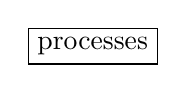
\begin{tikzpicture}
      \node [rectangle, text centered, draw=black]{processes};
    \end{tikzpicture},
    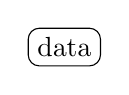
\begin{tikzpicture}
      \node [rectangle, rounded corners, text centered, draw=black]{data};
    \end{tikzpicture} and
    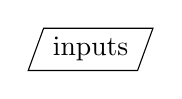
\begin{tikzpicture}
      \node [trapezium, trapezium left angle=70, trapezium right angle=110,
             text centered, draw=black]{inputs};
  \end{tikzpicture}}
  \label{figure:flow_chart}
\end{figure}

\section{Application}
\label{sec:application}

We have applied our methodology to evaluating QuickSpec, %TODO:cite
a library for conjecturing equations about functions written in the Haskell
programming language. We use the Tons of Inductive Problems (TIP) theorem
proving benchmark to generate our corpus.

\subsection{QuickSpec}

We use QuickSpec version 0.9.6 to demonstrate our benchmarking methodology. This
is a Haskell library which takes a \emph{signature} containing Haskell functions
and (universally quantified) typed variables, and outputs conjectured equations
involving these terms.

The QuickSpec algorithm first enumerates all well-typed expressions up to a
certain depth (3 by default), involving the given terms. Expressions of the same
type are assumed to be equivalent, and grouped into equivalence classes. A
testing process then tries to disprove this assumption by instantiating each
variable with a randomly chosen value (using the QuickCheck testing library),
evaluating the expressions and comparing the results. The equivalence classes
are split to separate any expressions which are observed to be different, and
the process repeats with new random values.

After 500 rounds of testing, any expressions still sharing the same equivalence
class are conjectured to be equal. Finally, a congruence closure algorithm is
applied to these equations, to find a minimal set.

In order to thoroughly benchmark QuickSpec, we need to automate some of the
decisions which are normally left up to the user:

\begin{itemize}
\item We must decide what variables to include. We add three for each type that
  appears as a function argument, except for types which have no QuickCheck data
  generator.
\item We must \emph{monomorphise} all types. For example, functions like
  \texttt{cons} are \emph{polymorphic}: they build lists of any element type.
  We need to pick a specific type in order to generate random values, so we
  resolve this (arbitrarily) by picking
  \texttt{Integer}.~\footnote{We pick \texttt{Integer} for variables of kind
    \texttt{*}, and \texttt{[]} (Haskell's list type constructor) for those of
    kind \texttt{* -> *}. If these violate some constraint, we pick a suitable
    type non-deterministically from the module scope, or skip these variables
    completely if none is found.}
\item Haskell functions only take one argument, as as in the $\lambda$-calculus,
  so functions of multiple arguments are simulated by currying.
  Unfortunately QuickSpec cannot compare functions for equality, so we must give
  each function in our signature an explicit arity. Arities from zero to five
  are supported, so we avoid partial application by picking the highest that is
  type-correct.
\end{itemize}

To find out which functions to include in a signature, we use a plugin for the
GHC compiler which tells us all of the functions defined in a package. We
include all of those which type-check when passed to QuickSpec.

\subsection{TIP}

We chose TIP for our ground truth since it satisfies the desiderata of
section~\ref{section:prep}: each problem has standalone type and function
definitions, making their separation trivial; known examples from the software
verification and inductive theorem proving literature are included, ensuring
relevance to those fields; the format includes higher-order functions and
inductive datatypes, which we are interested in; plus it is accompanied by
tooling to convert this format into a variety of languages, including Haskell
and Isabelle.

We use TIP version 0.2 which contains 343 problems, each stating a single
theorem and together defining a total of 618 datatypes and 1498 functions. Most
of these are duplicates, since each problem (re\nobreakdash-)defines all of the
datatypes and functions it involves. To avoid ambiguity we prefix the names of
all definitions with the filename it came from, and collect them into one big set.

TIP datatypes can have several ``constructors'' and ``destructors''. For example
the type of lists from figure~\ref{figure:list_theory} can be defined in TIP as
follows:

\begin{verbatim}
(declare-datatypes (a) ((List (Nil) (Cons (head a) (tail (List a))))))
\end{verbatim}

This defines a type \texttt{List} parameterised by a type variable \texttt{a}
(the type of the list's elements), with constructors \texttt{Nil} and
\texttt{Cons}, and destructors \texttt{head} and \texttt{tail}. Target languages
(e.g. Haskell and Isabelle) handle constructors and destructors differently, so
we avoid exploring them directly. Rather, we $\eta$-expand each constructor and
destructor to create new function definitions, and rewrite the TIP theorems to
reference these expanded forms instead.

TIP has ``native'' support for booleans and integers, allowing functions like
\texttt{+} to be used without an accompanying definition. To ensure consistency
in the translations, we replace all occurrences of these ``native'' expressions
with standard definitions using the same \texttt{declare-datatypes} and
\texttt{define-fun} mechanisms as the problem set.

This gives us a total of 3598 definitions, including those from the problem set
and our automatically-generated additions. Removing $\alpha$-equivalent
duplicates leaves 269 definitions, and we chose to only sample from those 182
which occur in at least one theorem statement (this removes ambiguity about
which \emph{definitions}, including our generated ones, are ``interesting'' and
which are just ``implementation details'').

TIP includes a tool to translate its definitions into Haskell code, including
suitable comparison functions and random data generators. We translated all 269
definitions into a single Haskell package, compiled it with GHC and extracted
the function definitions with our plugin. Each benchmark run imported this
entire package, but the signature given to QuickSpec only included functions
chosen for the current sample.

\subsection{Results}

\begin{figure}
  \centering
  \input{time.pgf}
  \caption{Running times of QuickSpec on theories sampled from TIP. Each point
    is an individual run, with 30 per size except for 1 (14) and 2 (29). Colour
    indicates the total number of conjectures produced by each run, with failing
    processes shown in red. Some points are shifted horizontally to prevent
    overlaps. Standard box plots are included, although many are obscured due to
    quartiles near zero or timeout. Whiskers show points at 1.5 $\times$ the
    inter-quartile range.}
  \label{figure:quickspec_runtimes}
\end{figure}

\begin{figure}
  \centering
  \input{prec.pgf}
  \caption{Precision and recall of all runs (spread horizontally to avoid
    overlaps). Point colour shows how many conjectures were in the ground truth
    set for each run. Lines show the mean value (average of ratios) and the
    shaded region is standard deviation, assuming a binomial distribution.}
  \label{figure:quickspec_precRec}
\end{figure}

We applied our sampling methodology to the 269 TIP definitions for sample sizes
between 1 and 20. We chose 30 samples for each size, but due to the requirement
for samples to admit at least one theorem, only 14 unique samples were obtained
for size 1 and 29 for size 2. A timeout of 3 minutes was imposed, since
preliminary experiments showed that most runs either finish before this time, or
still do not finish after an hour. The running times are shown in
figure~\ref{figure:quickspec_runtimes}.

The only errors we encountered were timeouts (shown in red), and these occurred
for all sample sizes. Whilst the median runtimes are mostly in the range of a
few seconds, the variance shows two distinct regions: sizes below 10 are mostly
finished within 30 seconds, whilst sizes 10 and above have large variance; the
whole upper quartile of size 13 timed out. There is also an unexpected downwards
trend towards size 20, and a slight but consistent reduction in minimum runtimes
from sizes 15 to 20 which is likely an artefact of our testing setup.

Most runs finished quickly and generated few conjectures, with the most being
131 conjectures from a sample of size 20.

Equations generated by QuickSpec and those from the ground truth were normalised
by numbering their variables and putting the left- and right-hand-sides in
lexicographical order. These two sets were then compared syntactically for
precision and recall, with the results shown in
figure~\ref{figure:quickspec_precRec}.

We use a binomial distribution to model precision and recall, as if each
conjecture is a ball drawn from an urn of wanted/unwanted results (in the case
of precision) or found/missed ground truths (in the case of recall). The mean of
these distributions estimates the overall proportion of wanted or found
conjectures, and we use the standard deviation to determine how well this mean
fits the data.

There is a clear negative trend in precision as the sample size increases,
indicating that a more aggressive post-processing filter may be useful as we
explore larger theories. Some small samples reached full precision, but nothing
above size 10 exceeded 50\%.

Recall shows a slight downward trend but is mostly flat, averaging between 10\%
and 40\%. This is expected, since adding more definitions to a QuickSpec
signature will never reduce the conjectures it will find. Those conjectures
which QuickSpec failed to find include terms which QuickSpec cannot synthesise
(such as conditional equations, inequalities, terms larger than the search depth
and those with anonymous functions) as well as equations which are removed as
``uninteresting'' by the final congruence closure step.

% Altogether TIP problem by QuickSpec and IsaCoSy theory
% exploration systems. To assess the scalability of their algorithms, we sampled
% theories of various sizes: from theories containing only a single definition, up
% to theories containing 20 definitions.
%  We call the Theory Exploration Benchmark (TEB).

% To do this we can take a set of ATP tasks, for example proving the equation
% \ref{eq:mapreduce} from the theory in figure \ref{figure:list_theory}, and we
% split apart the definitions (to form a theory) from the theorem statements (to
% form our ground truth).

% We focus on the Tons of Inductive Problems (TIP) theorem proving
% benchmark~\cite{claessen2015tip}, since it has several desirable properties:

% All together, TIP provides 219 distinct function definitions and 343
%   theorem statements, which is enough to fully exercise current MTE systems.
% Benchmark problems include examples from the theorem proving literature
%   as well as common program verification tasks, ensuring the resulting corpus is
%   relevant to researchers and practitioners.
% TIP's maintainers provide a set of tools, including translators from TIP's
%   native format (based on SMT-Lib~\cite{BarFT-SMTLIB}) to Haskell and Isabelle
%   (which are used by MTE systems).

% To aid reproducibility, we use a cryptographic hash as our source of randomness:
% the $n$th sample of size $s$ uses the SHA256 hash of $n$, $s$ and the definition
% corpus; the latter prevents tailoring the corpus to influence the choices,
% although MTE systems could .

% To provide a more robust comparison of these two systems, we also applied a
% paired difference test: measuring, for each sampled theory, the difference in
% time, precision and recall between the two systems.

\section{Discussion}
\label{sec:discussion}

The key to our benchmarking methodology is the simplifying assumption that
theorem proving problem sets are a good proxy for desirable MTE output. This
allows us to side-step the philosophical quagmire of ``interestingness'' to
produce concrete, measurable values; it is also a core weakness, as there are
compelling reasons to refute it.

Fundamentally, any mathematical reasoning system must decide on, and formalise,
what counts as ``the good'' in mathematics.  Obvious metrics such as ``true'' or
``provable'' include trivial tautologies, while at the same time failing to
capture the ``almost true'', which can be a valuable trigger for theory change,
as demonstrated by Lakatos in his case studies of mathematical
development~\cite{lakatos}. ``Beautiful'' is another -- albeit vague -- commonly
proposed metric. Methods for finding out what that means have come from
neuro-scientists, such as the study by Zeki \etal{} in which they test whether
mathematicians' experiences of abstract beauty correlates with the same brain
activity as experiences of sensory beauty~\cite{zeki}; computer scientists, such
as Colton's metrics above which are proposed based largely on a computer
scientist's ``intuition'' and argumentation about why a metric would be
important (and previous use of such metrics, and - in one isolated case
(surprisingingness) - on a single quote from a mathematician\footnote{Similarly,
  classification of a MATHsAiD result as either interesting or
  uninteresting~\cite{roy} was made by the main system developer: in both cases
  the main developer had a background in mathematics.}; and mathematicians
themselves, such as Gowers' suggestion that we can identify features which are
commonly associated with good proofs~\cite{gowers}. All of these approaches rest
upon the assumption that it makes sense to speak of ``the good'' in mathematics.
This assumption is supported by concepts such as Erdos's ``The Book'' -- a
theoretical construct of a book which contains the most elegant proof of every
theorem (brought to life in~\cite{aigner2010proofs}). However, empirical studies
by psychologists such as Inglis call into question such assumptions: work by
Inglis and colleagues has shown that there is not a single standard of validity
among contemporary mathematicians %FIXME https://dspace.lboro.ac.uk/dspace-jspui/handle/2134/12150
nor beauty. %FIXME needs citation

We do not claim that our use of corpora as a ground truth exactly captures all
interesting conjectures of their definitions, or that those definitions exactly
represent all theories we may wish to explore. Rather, we consider our approach
to offer a pareto-optimal balance between theoretical rigour and experimental
practicality, at least in the short term. Futhermore, since research is already
on-going in these areas, we hope to at least improve on existing evaluation
practices and offer a common ground for future research.

Notably, if MTE matures to the point of providing \emph{truly novel} insights,
even in well-studied domains, then the assumptions we rely on break down because
such results cannot (by definition) appear in any existing corpus.

Another practical limitation limitation of our benchmarking approach is that it
only applies to systems which act in ``batch mode'', i.e. those which choose to
halt after emitting some output. Whilst all of the systems we have encountered
are of this form, an analogous benchmark may be desirable for systems which
instead run continuously or interactively (perhaps akin to McCarthy's
``advice taker''~\cite{McCarthy_Programs59}).

% philosophical bits

% We're assuming there is general agreement on what is "good maths", when
% actually this isn't at all clear-cut

% agreement in maths? matt inglis

% other - zeki/two papers with ursula...

% methodology behind Simon's paper

\section{Conclusion}
\label{sec:conclusion}

% future work, etc.

Our benchmarking methodology, and accompanying suite based on TIP, provides a
general way to evaluate and compare many diverse approaches to the problem of
theory exploration, whilst avoiding some of the philosophical complications of
the field. The methodology can be adapted to suit particular domains, for
example our experiments have focused on inductive theories with higher-order
functions, and the corpora used to generate a benchmark suite can always be
improved and refined with the addition of new definitions and theorems.

We believe that a standard approach to benchmarking and comparison will ease the
burden on researchers wanting to evaluate systems, and provide a common goal to
pursue in the short term.

``Solving'' this benchmark suite would not solve the problem of theory
exploration in general, so more ambitious goals must be set in the future; but
we believe that our approach will provide a compelling challenge, at least for
the foreseeable future.

%\begin{acknowledgements}
%  We are grateful to Jianguo Zhang for help with our statistical analysis.
%
%  EPSRC
%\end{acknowledgements}

\bibliographystyle{plain}
\bibliography{./Bibtex}

\end{document}
